

    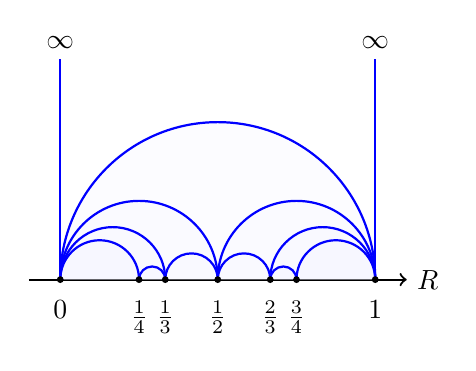
\begin{tikzpicture}[scale=4, thick]
        
        % 1. 画实轴 (边界)
        \draw[->, thick] (-0.1, 0) -- (1.1, 0) node[right] {$\mathbb{R}$};
        
        % 2. 画通向无穷远点的垂直测地线 (从 0 和 1 出发)
        \draw[blue] (0, 0) -- (0, 0.7) node[above, text=black] {$\infty$};
        \draw[blue] (1, 0) -- (1, 0.7) node[above, text=black] {$\infty$};
        
        % 定义一个绘制半圆的样式，统一颜色和线宽
        \tikzset{farey edge/.style={blue, fill=blue!5, fill opacity=0.2}}

        % 3. 逐层画出 Farey 三角形的边 (半圆)
        % 语法：\draw (右端点, 0) arc (0:180:半径);
        
        % F1 的边: 0/1 和 1/1
        \draw[farey edge] (1, 0) arc (0:180:1/2);
        
        % F2 的边: 引入 1/2
        \draw[farey edge] (1/2, 0) arc (0:180:1/4); % 0/1 -- 1/2
        \draw[farey edge] (1, 0) arc (0:180:1/4);   % 1/2 -- 1/1
        
        % F3 的边: 引入 1/3 和 2/3
        \draw[farey edge] (1/3, 0) arc (0:180:1/6);  % 0/1 -- 1/3
        \draw[farey edge] (1/2, 0) arc (0:180:1/12); % 1/3 -- 1/2
        \draw[farey edge] (2/3, 0) arc (0:180:1/12); % 1/2 -- 2/3
        \draw[farey edge] (1, 0) arc (0:180:1/6);    % 2/3 -- 1/1
        
        % F4 的边: 引入 1/4 和 3/4 (为了画面干净，省略 2/5 等其他内部细节)
        \draw[farey edge] (1/4, 0) arc (0:180:1/8);  % 0/1 -- 1/4
        \draw[farey edge] (1/3, 0) arc (0:180:1/24); % 1/4 -- 1/3
        \draw[farey edge] (3/4, 0) arc (0:180:1/24); % 2/3 -- 3/4
        \draw[farey edge] (1, 0) arc (0:180:1/8);    % 3/4 -- 1/1

        % 4. 标注实轴上的顶点
        \filldraw[black] (0, 0) circle (0.2pt) node[below=4pt] {$0$};
        \filldraw[black] (1, 0) circle (0.2pt) node[below=4pt] {$1$};
        \filldraw[black] (1/2, 0) circle (0.2pt) node[below=4pt] {$\frac{1}{2}$};
        \filldraw[black] (1/3, 0) circle (0.2pt) node[below=4pt] {$\frac{1}{3}$};
        \filldraw[black] (2/3, 0) circle (0.2pt) node[below=4pt] {$\frac{2}{3}$};
        \filldraw[black] (1/4, 0) circle (0.2pt) node[below=4pt] {$\frac{1}{4}$};
        \filldraw[black] (3/4, 0) circle (0.2pt) node[below=4pt] {$\frac{3}{4}$};
        
    \end{tikzpicture}
